\documentclass[12pt]{article}

\usepackage[numbers,sort]{natbib}
\usepackage{amsfonts, amsmath}
\usepackage{graphicx}
\usepackage{libertine}
\usepackage{fullpage}
\usepackage{hyperref}
\hypersetup{
    colorlinks = true,
    linkcolor = blue,
    urlcolor  = blue,
    citecolor = blue,
    anchorcolor = blue}
\urlstyle{same}
\usepackage{booktabs}
\usepackage{xcolor}
\usepackage{caption}
\usepackage{float}
\captionsetup{font=small}
\newcommand{\ci}[2]{\,[#1,\,#2]}

\begin{document}

\title{When does structure help? Bayesian optimisation versus CMA-ES under low effective dimension and rotation}
\date{}
\maketitle
{\bf Member:}
\begin{enumerate}\setlength{\itemsep}{0pt}
\item {Sufiya Najeeb, A0286567J}
\end{enumerate}

{\bf Github Repository:} https://github.com/ssufiya/dsa4211project (all numbers and figures in this report
are reproduced by the commands in \texttt{README.md})

\section{Introduction}
Black-box optimisation problems such as hyperparameter tuning often have many inputs of which only
a few matter: Bergstra and Bengio~\cite{bergstra2012random} found that for most of their neural-network tuning tasks
only a few hyperparameters were important, and that which ones mattered changed from dataset to
dataset. If an optimiser can discover such low-dimensional structure, it effectively searches a
much smaller space. Whether it can may depend on whether the important directions are individual
inputs (\emph{aligned}) or combinations of inputs (\emph{rotated}).

Bayesian optimisation and CMA-ES differ precisely in this aspect. CMA-ES is designed to be invariant
to rotations of the search space \cite{hansen2016cma}, while a Gaussian-process (GP) surrogate with
one lengthscale per input (an ARD kernel) can switch off irrelevant inputs but only along the
coordinate axes \cite{rasmussen2006gp}. TuRBO \cite{eriksson2019turbo} offers a middle ground, by applying local, axis-aligned bounding boxes that adapt to local landscape features without requiring full rotation invariance. This motivates three questions, which this project investigates: 

\begin{itemize}
  \item[\textbf{Q1}] Does rotating the relevant subspace change how well each method performs?
  \item[\textbf{Q2}] How does performance change with the ambient dimension $D$ and the effective
  dimension $d_e$?
  \item[\textbf{Q3}] Can the differences we observe be explained by the methods' invariance
  properties and by what each must learn from data?
\end{itemize}
We report what we found for each method, use diagnostics recorded during the runs to explain it, and
then investigate the results we did not expect (Section~\ref{sec:invest}).

\section{Background}
\paragraph{Bayesian optimisation.} BO fits a probabilistic surrogate of the objective, usually a GP,
and chooses each new point by maximising an acquisition function that trades off a low predicted
value against high uncertainty \cite{frazier2018tutorial}. We use Expected Improvement
\cite{jones1998ego}, evaluated in log space for numerical stability \cite{ament2023logei}. The GP's
kernel controls how quickly the modelled function may vary. A Mat\'ern kernel with a single shared
lengthscale is unchanged under rotations of the inputs. An \emph{automatic relevance determination}
(ARD) kernel has one lengthscale $\ell_i$ per input; a very long $\ell_i$ means the model treats the
function as constant along input $i$. ARD therefore reduces the effective dimension of the model,
but only for directions that coincide with coordinate axes.

\paragraph{CMA-ES.} CMA-ES samples a population from a multivariate Gaussian, ranks the candidates by
objective value, and moves the mean towards the best while adapting the step size and the full
covariance matrix \cite{hansen2016cma}. Because it uses only ranks and a full covariance, it is
invariant to monotone transformations of the objective and, when unconstrained, to rotations of the
search space: a rotated problem started from correspondingly rotated initial conditions produces
the same sequence of objective values. The price is that the covariance has about $D^2/2$ entries,
so its learning rate falls roughly as $1/D^2$, and adapting to the problem's shape becomes slow in
high dimension.

\paragraph{Trust-region BO.} Eriksson et al.~\cite{eriksson2019turbo} argue that a single global GP struggles in high
dimension because it is implicitly homogeneous and the acquisition over-explores. TuRBO instead fits
a GP and samples only inside a trust region around the best point. The region is a box whose side
lengths are proportional to the ARD lengthscales, normalised to a target volume. It doubles after
three consecutive improvements, halves after $\max(4,D)$ consecutive failures, and the run restarts
when it collapses. New points are chosen by Thompson sampling. We implement TuRBO-1 (a single trust
region), whose axis-aligned box makes it directly relevant to our question.

\paragraph{Random search and benchmarking.} Bergstra and Bengio~\cite{bergstra2012random} showed that random search
matched or beat grid search and carefully hand-tuned settings for neural networks in a fraction of the
time, and explained this by low effective dimension: random points explore many distinct values of
each important input, whichever inputs those turn out to be. They conclude that random search is a
natural baseline for judging adaptive methods. This matters especially here: since low effective
dimension already favours random search, a method only demonstrates that it exploits the structure
if it clearly beats this baseline. We follow COCO \cite{hansen2021coco} in measuring performance by
the number of objective evaluations, using many problem instances and runtime distributions over
target values.

\section{Experimental setup}
\subsection{Test problems}
Each problem is defined on the box $\mathcal{X}=[-1,1]^D$ as
\begin{equation}
  f(x) = g\!\left(A^\top x - z^\star\right) + \varepsilon\,\big\|(I - AA^\top)(x - x^\star)\big\|^2,
  \label{eq:problem}
\end{equation}
where $A\in\mathbb{R}^{D\times d_e}$ has orthonormal columns and $g$ is a base function on
$\mathbb{R}^{d_e}$ with minimum value $0$ at the origin. We use Ackley, which has many local minima on
a global funnel, and Rosenbrock, a narrow curved valley; both are classical COCO functions and test
different difficulties. They are rescaled so their interesting region fits the box. The optimum
$x^\star$ is drawn uniformly from $[-0.5,0.5]^D$ and $z^\star = A^\top x^\star$, so the global minimum
$f(x^\star)=0$ lies inside the box and $f(x)$ is exactly the \emph{simple regret}. In the
\emph{aligned} case $A$ selects $d_e$ random coordinates; in the \emph{rotated} case $A$ is the
orthonormal factor of a Gaussian matrix. The base function, $d_e$ and the box are identical; only the
orientation of the relevant subspace changes. A seed determines the instance ($A$, $x^\star$) and
the initial design, and every method sees the same instance for a given seed. The parameter
$\varepsilon$ is zero except in Section~\ref{sec:approx}.

\subsection{Methods and protocol}
Table~\ref{tab:methods} lists the methods. All methods first evaluate the same 10-point Latin
hypercube design; CMA-ES then starts from its best point and TuRBO centres its first trust region
there. All methods use default settings, with no per-problem tuning. The GP-BO and isotropic GP
methods form a controlled pair that differs only in the kernel's lengthscales, so any difference in
their sensitivity to rotation can be attributed to ARD.

\begin{table}[h]
\centering\small
\begin{tabular}{p{2.5cm}p{3.6cm}p{9.2cm}}
\toprule
Method & Implementation & Settings \\
\midrule
Random search & own & Latin hypercube, then uniform random points \\
CMA-ES & pycma \cite{hansen2019pycma} & $\sigma_0=0.5$ (a quarter of the box width), default population $4+\lfloor 3\ln D\rfloor$, pycma bound handling, restart from a random point on a stopping criterion \\
GP-BO (ARD) & scikit-learn \cite{pedregosa2011sklearn} & Mat\'ern-5/2, one lengthscale per input in $[0.01,100]$, log EI maximised over 5000 uniform candidates plus local perturbations of the best points \\
GP-BO (isotropic) & scikit-learn & as ARD, with one shared lengthscale \\
TuRBO-1 & own, following Eriksson et al.~\cite{eriksson2019turbo} & paper defaults (side length $0.8$, minimum $2^{-7}$, maximum $1.6$, lengthscales $\le 2$ on the unit cube); Thompson sampling over $\le 2000$ candidates \\
\bottomrule
\end{tabular}
\caption{Methods compared. Exact settings are in \texttt{configs/} and \texttt{code/methods.py}.}
\label{tab:methods}
\end{table}

\paragraph{Budget and measures}
The budget is the number of objective evaluations, including the
initial design: 200 in the main experiments and 3000 for CMA-ES and random search in a follow-up
(GP methods are too slow at that budget). Wall-clock time is reported separately. Our measure is the
$\log_{10}$ simple regret of the best point found, so a difference of 1 means a factor of 10. We report
medians and interquartile ranges over 15 seeds per setting, matching the 15 instances per function used
by COCO. The central quantity is the \emph{rotation effect}: the median log regret on rotated instances
minus that on aligned instances, with a bootstrap 95\% confidence interval over seeds. A positive value
means the method is worse when rotated. Comparisons between methods are paired by seed, since both
face the same instance and initial design. Because the evaluations are noise-free, the best observed
value is the true regret of the recommended point.

\paragraph{Pilot}
A pilot (100 evaluations, 5 seeds, $D\in\{10,30\}$) showed rotation effects for ARD-GP but almost no
covariance adaptation by CMA-ES, so we raised the main budget to 200, used 15 seeds, and added a
long-budget CMA-ES follow-up. In the pilot, random search appeared much better on rotated than aligned Rosenbrock
at $D=30$ (median difference $-1.16$ orders of magnitude), although with only 5 seeds
the 95\% interval $\ci{-1.68}{0.73}$ already included zero. With 15 seeds the
difference vanished ($+0.17\ci{-0.39}{0.53}$), confirming it was due to chance.

\section{Results}
\subsection{Effect of rotation (Q1)}
\begin{figure}[H]
\centering
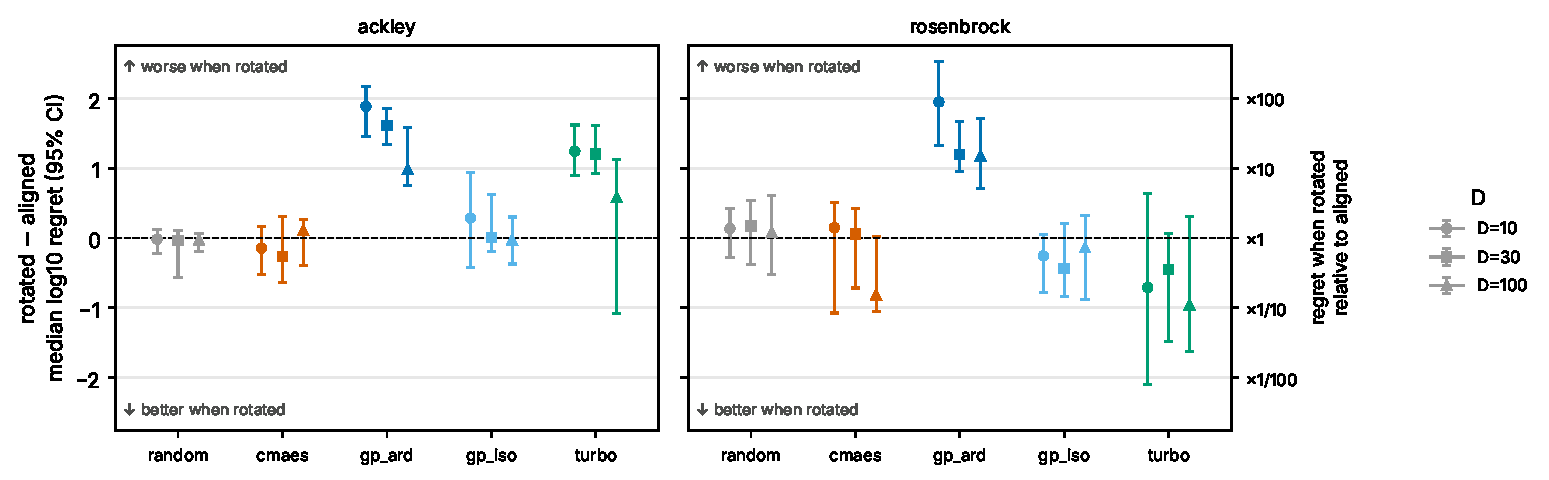
\includegraphics[width=0.9\linewidth]{figures/main_dimension_rotation_effect.pdf}
\caption{Rotation effect (rotated minus aligned median $\log_{10}$ regret after 200 evaluations) with
bootstrap 95\% CIs, $d_e=2$, 15 seeds. Above the dashed line: worse when rotated; the right axis
gives the same values as the ratio of rotated to aligned regret.}
\label{fig:rot}
\end{figure}

Figure~\ref{fig:rot} summarises the main experiment (the values are in
\nolinkurl{results/main_dimension/summary_rotation_effect.csv}). We describe three findings.

\paragraph{Finding 1: GP-BO with ARD exploits aligned structure and loses this advantage under
rotation.} GP-BO with ARD is clearly worse on rotated problems in all six settings, by a factor between
about 10 and 90; every confidence interval lies above zero. The isotropic GP, identical except for its
single lengthscale, shows no clear effect anywhere, and neither does random search, so the problems
themselves are not harder when rotated. The difference between the two GP variants isolates the
per-input lengthscales as the cause, which is consistent with how ARD works (Section~2): it can only
switch off directions that coincide with an input. The diagnostics show this directly: in
\emph{every} aligned setting, the two shortest ARD lengthscales were exactly the two relevant inputs
(\texttt{relevant\_recovered\_frac}$\,=1.0$), while almost all irrelevant inputs (97\% on average) reached the upper bound of 100.
On aligned problems this made ARD-GP the best method overall: it beat CMA-ES on 15 of 15 seeds in five
of the six settings (14 of 15 on Rosenbrock, $D=30$), by 1.2 to 2.5 orders of magnitude. On rotated
Rosenbrock it was no better than CMA-ES (paired differences $+0.15$, $+0.20$, $+0.26$, all intervals
containing or touching zero).

\paragraph{Finding 2: CMA-ES is unaffected by rotation, but had learned little within 200 evaluations.}
CMA-ES shows no clear rotation effect, consistent with its rotation invariance \cite{hansen2016cma};
the borderline case is Rosenbrock with $D=100$ ($-0.82\ci{-1.05}{0.02}$), where it was if anything
better when rotated. However, this says little on its own, because the diagnostics show that CMA-ES
had barely adapted its search distribution. For $D\ge 30$, the fraction of its covariance's variance
lying in the relevant subspace stayed at the value $d_e/D$ of a round (isotropic) distribution
(e.g.\ $0.020$ versus $0.020$ at $D=100$), and the covariance's condition number was below 2. Only at
$D=10$ had it adapted modestly (fraction $0.08$--$0.15$ versus $0.20$, condition number 5--7). On
Rosenbrock it did not significantly beat random search in any setting. An optimiser that has not yet
learned the problem's shape cannot be affected by its orientation, so this absence of a rotation
effect is weak evidence for invariance. Section~\ref{sec:long} therefore gives CMA-ES 3000 instead of
200 evaluations.

\paragraph{Finding 3: TuRBO behaves like ARD-GP on Ackley but not on Rosenbrock.} TuRBO's trust region is
an axis-aligned box shaped by ARD lengthscales, and on Ackley it is clearly worse when rotated for
$D=10$ and $30$ ($+1.24$ and $+1.20$), like ARD-GP. On Rosenbrock, however, the effect points the
other way in all three settings, although no interval excludes zero. We did not expect this;
Section~\ref{sec:turbo} investigates it.

\subsection{Effect of ambient dimension (Q2)}
Increasing $D$ from 10 to 100 reduces ARD's advantage on aligned Ackley
(median log regret $-2.71$, $-2.37$, $-1.94$) and TuRBO's even more ($-2.65$, $-1.93$, $-0.95$).
TuRBO's trust region shrinks only after $\max(4,D)$ consecutive failures, so at $D=100$ it shrank at most
once within 200 evaluations (median final side length $0.8$ on aligned Ackley) and behaved almost
like a fixed local search. Figure~\ref{fig:finalD} in the appendix shows final regret against $D$.

\subsection{Long-budget CMA-ES}\label{sec:long}
\begin{figure}[t]
\centering
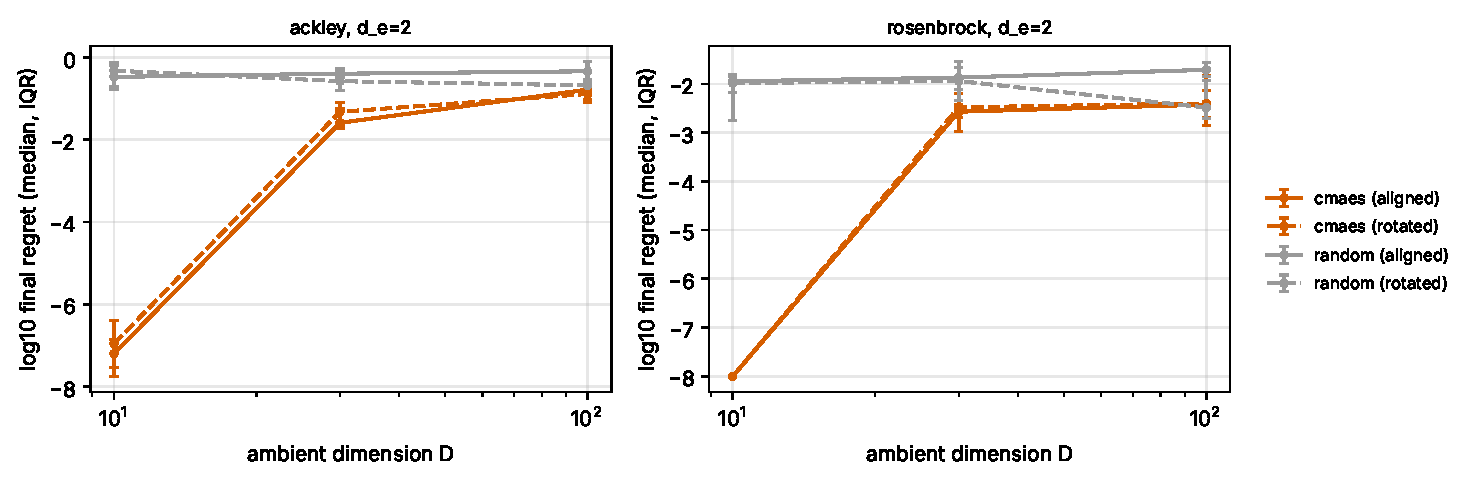
\includegraphics[width=0.78\linewidth]{figures/followup_cmaes_long_final_vs_D.pdf}\\[2pt]
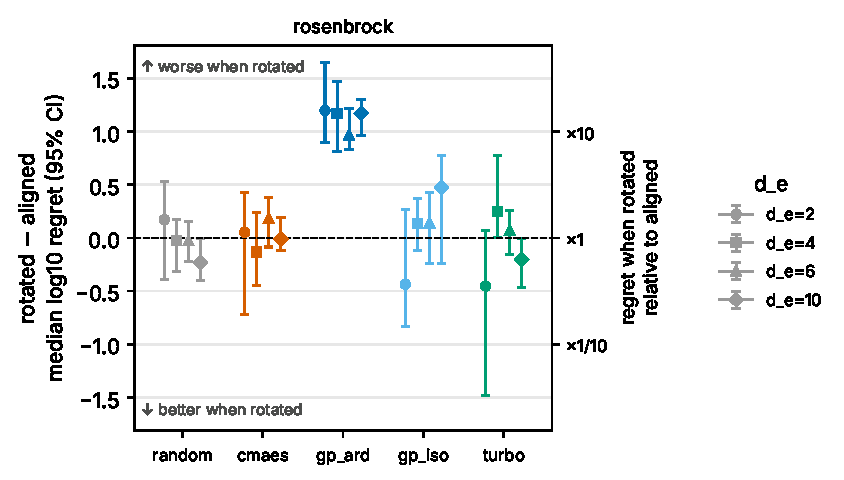
\includegraphics[width=0.49\linewidth]{figures/main_effective_dim_rotation_effect.pdf}\hfill
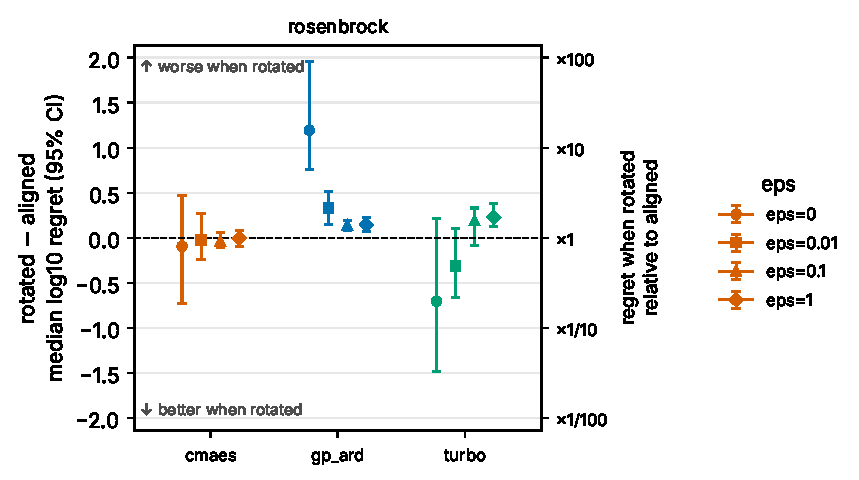
\includegraphics[width=0.49\linewidth]{figures/followup_approx_lowdim_rotation_effect.pdf}
\caption{Follow-up experiments. Top: final $\log_{10}$ regret of CMA-ES and random search after 3000
evaluations against $D$ (solid aligned, dashed rotated; median and IQR). Bottom: rotation effect on
Rosenbrock with $D=30$ as the effective dimension $d_e$ grows (left) and as the remaining directions
start to matter, $\varepsilon>0$ (right).}
\label{fig:followups}
\end{figure}
With 3000 evaluations (Figure~\ref{fig:followups}, top), CMA-ES reaches a median $\log_{10}$ regret of
$-7.2$ on Ackley at $D=10$ (Rosenbrock reaches the analysis floor of $10^{-8}$), far below any method at
200 evaluations, but only $-1.6$ to $-2.6$ at $D=30$ and $-0.8$ to $-2.4$ at $D=100$. This strong
dependence on $D$ matches its slow, $O(D^2)$ covariance learning (Section~2). Its rotation effect remains
indistinguishable from zero in all six settings (e.g.\ Ackley $D=30$: $+0.27\ci{-0.18}{0.52}$), now for a
method that has clearly adapted (condition number above $10^7$ at $D=10$).

However, the search distributions it learned were not the same. At $D=10$, the fraction of variance in
the relevant subspace was $0.000$ on aligned problems but $0.09$--$0.12$ on rotated ones, despite
similar regret (\texttt{results/investigations.txt}). The box and pycma's way of keeping points inside
it are the only axis-aligned parts of our setup, so they are the likely cause: CMA-ES reached the same
results in both cases, but by learning differently shaped search distributions.

\subsection{Effect of effective dimension (Q2)}
With $D=30$ and $d_e\in\{2,4,6,10\}$ (Figure~\ref{fig:followups}, bottom left), ARD-GP's rotation effect remains large and significant at every
$d_e$ ($+1.20$, $+1.17$, $+0.97$, $+1.17$; all intervals above $0.8$). Even at $d_e=10$, 20 of the 30
inputs are irrelevant, so ARD still has many inputs to switch off when the structure is aligned. All other methods show effects within about $\pm0.5$. The regret of every method
rises steeply with $d_e$, partly because Rosenbrock sums more terms as $d_e$ grows, so we compare
methods within each $d_e$ rather than across.

\subsection{Approximately low-dimensional problems}\label{sec:approx}
Real problems are rarely exactly low-dimensional. Setting $\varepsilon>0$ in \eqref{eq:problem} makes
the remaining 28 directions matter slightly ($D=30$, $d_e=2$, 10 seeds; Figure~\ref{fig:followups}, bottom right). ARD-GP's rotation effect falls from
$+1.20\ci{0.76}{1.96}$ at $\varepsilon=0$ to $+0.33\ci{0.15}{0.52}$ at $\varepsilon=0.01$ and about
$+0.15$ at $\varepsilon\in\{0.1,1\}$, and its aligned advantage over CMA-ES shrinks from about one order
of magnitude ($-2.17$ vs $-1.14$) to almost none ($-0.04$ vs $0.09$ at $\varepsilon=0.1$). ARD's benefit
therefore depends on irrelevant inputs being exactly irrelevant: even a weak dependence on all inputs
prevents it from switching them off. CMA-ES shows no rotation effect at any $\varepsilon$.

\subsection{Computational cost}\label{sec:cost}
\noindent\begin{minipage}[t]{0.54\linewidth}
\vspace{0pt}
CMA-ES needed under $0.1$\,s per 200-evaluation run at every $D$, whereas the GP-based methods needed
$18$--$48$\,s (isotropic GP), $22$--$195$\,s (TuRBO) and $62$--$680$\,s (ARD-GP), growing with $D$
(Figure~\ref{fig:time}). ARD-GP thus spends roughly $10^4$ times more computation per evaluation than
CMA-ES, mostly fitting $D+2$ kernel hyperparameters. This overhead is only worthwhile when each
objective evaluation is much more expensive and the structure is aligned; on rotated Rosenbrock
ARD-GP was no better than CMA-ES.
\end{minipage}\hfill
\begin{minipage}[t]{0.43\linewidth}
\vspace{0pt}
\centering
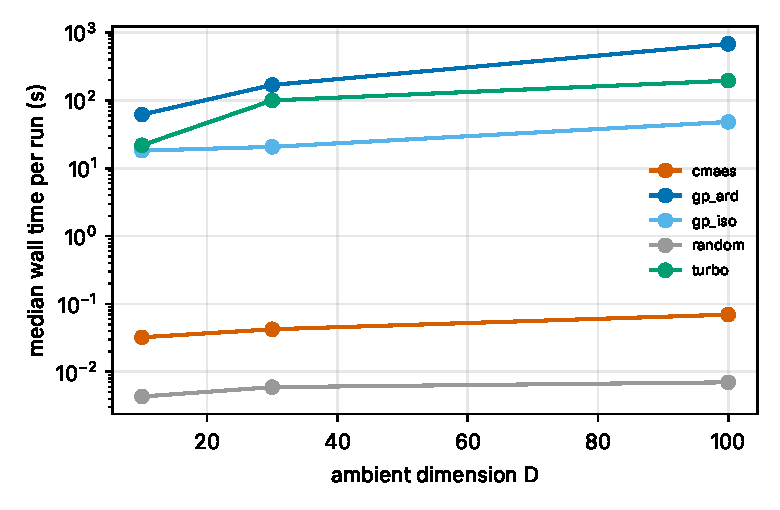
\includegraphics[width=\linewidth]{figures/main_dimension_walltime.pdf}
\captionof{figure}{Median wall-clock time per 200-evaluation run against $D$ (log scale).}
\label{fig:time}
\end{minipage}

\section{Investigating unexpected results}\label{sec:invest}
\subsection{Why TuRBO does not inherit the rotation effect on Rosenbrock}\label{sec:turbo}
If TuRBO's sensitivity to rotation on Ackley comes from its ARD-shaped trust region, it should only
appear when its GP actually identifies the relevant inputs. We checked the final lengthscales of all aligned
runs. Following the paper, TuRBO bounds lengthscales by $2$ on the unit cube, whereas our ARD-GP allows
up to $100$. On aligned Rosenbrock, in 20 of 45 TuRBO runs one of the two relevant inputs ended
\emph{at} the upper bound, indistinguishable from the irrelevant inputs, which all sit at the bound.
On aligned Ackley this never happened (0 of 45), and ARD-GP never hit its own bound on a relevant
input. Rosenbrock varies slowly along its valley, so one relevant input genuinely has a long
lengthscale: in the ARD-GP runs we inspected it was about $1.7$--$5$ on $[-1,1]$, comparable to
TuRBO's cap (2 on the unit cube, i.e.\ 4 on $[-1,1]$). TuRBO
therefore could not shape its box to exploit the aligned structure on Rosenbrock, had no advantage to
lose under rotation. This matches exactly where TuRBO's rotation effect disappears. This explanation is consistent with the
diagnostics but not yet tested causally; rerunning TuRBO with a larger lengthscale bound is the
natural next experiment.

\subsection{The box makes rotated problems different}\label{sec:box}
Rotation invariance is a property of unconstrained problems. Our box is axis-aligned, so rotating
the subspace also changes how the box looks from inside it. For $x$ uniform on $[-1,1]^D$, a relevant
coordinate $z=a^\top x$ is uniform on $[-1,1]$ when aligned, but a sum of many small contributions
when rotated, so it is close to Gaussian with the same variance $1/3$. The rotated distribution puts
more mass near the centre, where the optimum tends to lie: $P(|z|<0.25)$ is $0.25$ when aligned
but $0.32$--$0.33$ when rotated for $D\in\{10,30,100\}$. So uniform sampling should land near
the optimum more often on rotated problems. Our random-search control confirms it where the budget is
large enough to resolve it: with 3000 evaluations at $D=100$, random search was significantly better on
rotated problems for both functions ($-0.34\ci{-0.59}{-0.09}$ on Ackley, $-0.78\ci{-1.08}{-0.23}$ on
Rosenbrock), although no optimiser adapts to anything. The same geometry may contribute to the
negative rotation effects of CMA-ES and TuRBO on Rosenbrock at $D=100$, and it is why a structure-blind
control is needed to interpret any rotation effect.

\section{Discussion}
\paragraph{Q1: Does rotation matter?} Rotation matters only for methods whose notion of relevance is
tied to the coordinate axes. ARD-GP gives each input its own lengthscale; on aligned problems it
identified the relevant inputs in every run and gained one to two orders of magnitude, and rotating
the same problem removed this gain (10--90 times higher regret). The isotropic GP, identical except
for one shared lengthscale, and CMA-ES, whose covariance can point in any direction, were unaffected,
as was random search. TuRBO's trust region is shaped by ARD lengthscales, so it was affected on
Ackley; on Rosenbrock its capped lengthscales could not single out one relevant input, so it had no
aligned advantage to lose (Section~\ref{sec:turbo}). In practice, rotation invariance held only
approximately: CMA-ES's results were unaffected even after 3000 evaluations, but the search
distribution it learned was not, and the axis-aligned box made rotated problems slightly easier for
random search (Section~\ref{sec:box}).

\paragraph{Q2: How do ambient and effective dimension matter?} Dimension matters mainly through how much
each method has to learn. CMA-ES must adapt a covariance matrix with about $D^2/2$ entries: within 200
evaluations it had barely adapted for $D\ge 30$, and with 3000 it reached $\log_{10}$ regret below $-7$
at $D=10$ but only $-0.8$ (Ackley) and $-2.4$ (Rosenbrock) at $D=100$. TuRBO also slowed sharply as $D$
grew (aligned Ackley: $-2.65$ at $D=10$, $-0.95$ at $D=100$), because its trust region only shrinks after
$\max(4,D)$ consecutive failures. ARD-GP's aligned advantage shrank with $D$ but remained large, while on
rotated problems it was nearly flat in $D$. A larger effective dimension made every method much worse,
partly because Rosenbrock grows with $d_e$, yet ARD-GP's rotation effect stayed near one order of
magnitude up to $d_e=10$, since 20 of the 30 inputs were still irrelevant. Its advantage is fragile,
however: once the remaining directions mattered even slightly ($\varepsilon\ge 0.01$), it largely
disappeared, because no input could be switched off.

\paragraph{Q3: What explains the differences?} Taken together, \emph{each method's gain from low effective
dimension depends on whether its representation can express the orientation of the structure, and on
how much data it needs to learn it.} ARD-GP learns relevance quickly but only along the axes; CMA-ES can
represent any orientation but learns slowly. In practice, ARD-GP is the better choice when evaluations are
expensive enough to outweigh its overhead (Section~\ref{sec:cost}), the budget is small, and a few
individual inputs are expected to matter. CMA-ES is preferable when evaluations are cheap enough to
afford thousands, or when the important directions are likely to be combinations of inputs.

\paragraph{Limitations.} We used two synthetic base functions with mostly $d_e=2$, and GP methods only
up to 200 evaluations. Our GP-BO maximises the acquisition over a candidate set rather than by
gradient-based multi-start optimisation, and TuRBO uses at most 2000 Thompson-sampling candidates
instead of 5000, so absolute BO performance may be understated. All methods used default settings.
We did not include a non-rotation-invariant variant of CMA-ES (e.g.\ separable CMA-ES), so on the
evolution-strategy side we cannot isolate invariance as cleanly as with the two GP kernels. With 15
seeds, intervals on Rosenbrock are wide (about $\pm0.5$ to $\pm1$), so smaller effects cannot be
excluded. Evaluations were noise-free, timings come from a single laptop, and regrets below
$10^{-8}$ are floored in the analysis. The explanations in Section~5 are supported by diagnostics but
were not tested by intervention.

\section{Conclusion}
On problems with low effective dimension, GP-BO with an ARD kernel exploits structure that is aligned
with the input axes and outperforms CMA-ES by one to two orders of magnitude, but rotating the problem,
or letting the remaining inputs matter slightly, removes this advantage. CMA-ES is unaffected by
rotation but learns too slowly to exploit the structure within a BO-sized budget in high dimension.
Open questions are whether these conclusions hold on real, noisy problems, whether TuRBO behaves
differently with a larger lengthscale bound, and how much of CMA-ES's non-invariant adaptation is
caused by the box constraint.

\bibliographystyle{alpha}
\bibliography{references}

\appendix
\section{Additional figure}
\begin{figure}[!ht]
\centering
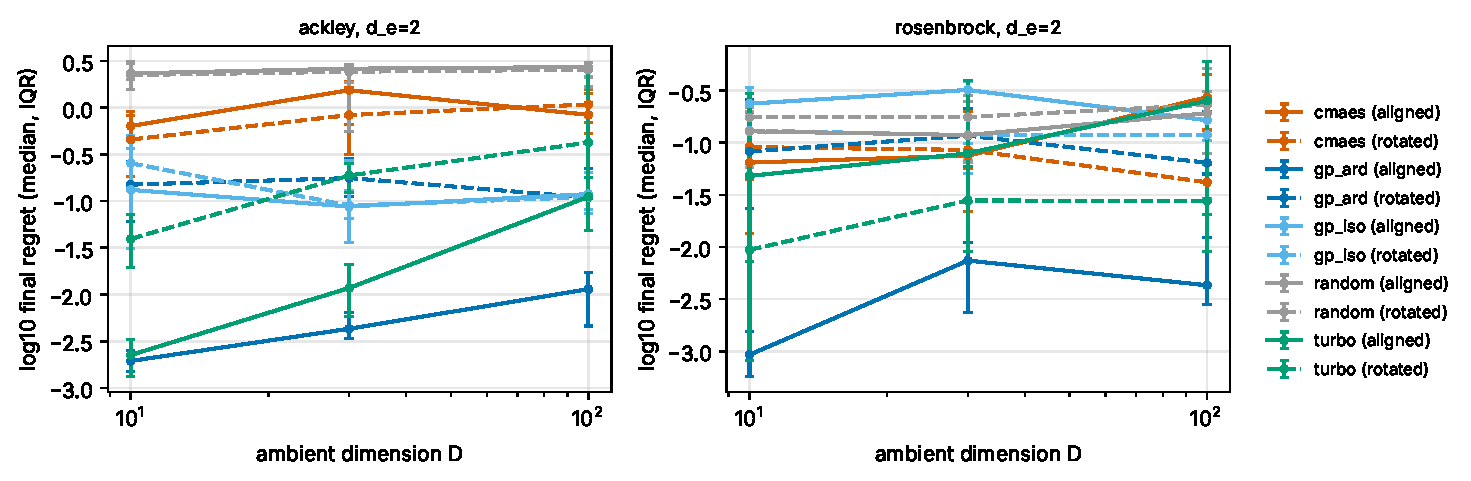
\includegraphics[width=0.66\linewidth]{figures/main_dimension_final_vs_D.pdf}
\caption{Final $\log_{10}$ regret after 200 evaluations against $D$ ($d_e=2$); solid aligned, dashed
rotated; median and IQR over 15 seeds.}
\label{fig:finalD}
\end{figure}
\end{document}
